% To je predloga za poročila o domačih nalogah pri predmetih, katerih
% nosilec je Blaž Zupan. Seveda lahko tudi dodaš kakšen nov, zanimiv
% in uporaben element, ki ga v tej predlogi (še) ni. Več o LaTeX-u izveš na
% spletu, na primer na http://tobi.oetiker.ch/lshort/lshort.pdf.
%
% To predlogo lahko spremeniš v PDF dokument s pomočjo programa
% pdflatex, ki je del standardne instalacije LaTeX programov.

\documentclass[a4paper,11pt]{article}
\usepackage{a4wide}
\usepackage{fullpage}
\usepackage[utf8x]{inputenc}
\usepackage[slovene]{babel}
\selectlanguage{slovene}
\usepackage[toc,page]{appendix}
\usepackage[pdftex]{graphicx} % za slike
\usepackage{setspace}
\usepackage{color}
\definecolor{light-gray}{gray}{0.95}
\usepackage{listings} % za vključevanje kode
\usepackage{hyperref}
\renewcommand{\baselinestretch}{1.2} % za boljšo berljivost večji razmak
\renewcommand{\appendixpagename}{Priloge}
\usepackage{subcaption}

\lstset{ % nastavitve za izpis kode, sem lahko tudi kaj dodaš/spremeniš
language=Python,
basicstyle=\footnotesize,
basicstyle=\ttfamily\footnotesize\setstretch{1},
backgroundcolor=\color{light-gray},
}

\title{Stiskanje in čiščenje slik s pomočjo DVT}
\author{David Rubin (david.rubin@student.um.si)}
\date{\today}

\begin{document}

\maketitle

\section{Uvod}

S pomočjo poljubne knjižnice izračunajte diskretno valčno transformacijo (DVT) slike. Izberite najprimernejši valček za vašo sliko. Število nivojev dekompozicije določite sami. Dobro preverite, kako so v izhodu DVT-ja zapisane podrobnosti in približki vhodne slike. 

Nad rezultatom DVT uporabite ali trdo ali mehko odstranjevanje motenj in visokih frekvenc, pri čemer testirajte različne pragovne vrednosti odstranjevanja. S pomočjo inverzne DVT spremenjene valčne koeficiente preslikajte nazaj v prostorsko domeno slik in jih primerjajte z originalno  sliko:
\begin{enumerate}
\item Testirajte vsaj štiri različne slike, ki naj bodo čimbolj različne. 
\item Vsaki sliki določite optimalni valček (testirajte vsaj tri različne valčke) in optimalen prag rezanja (testirajte vsaj štiri različne pragove rezanja). 
\item Ocenite stopnjo stiskanja in kvaliteto rekonstrukcije s pomočjo inverzne  DVT. Podobnosti oz. odstopanja med originalno in rekonstruirano sliko merite s korelacijskim koeficientom in normalizirano kvadratično napako (normalized root-mean-square deviation).
\item Za izbrane pragove rezanja ocenite razliko med mehkim in trdim pragovnim odstranjevanjem motenj. 
\item Postopke testiranja na izbrani sliki (lahko je ena sama) ponovite ob prisotnosti 20 dB belega šuma, ki ga tvorite sami.
\end{enumerate}

\section{Rezultati}

Za testiranje svoje rešitve sem si izbral 4 slike (slike~\ref{slika1}, ~\ref{slika2}, ~\ref{slika3} in ~\ref{slika4}). Testiral sem 5 različnih valčkov, ki so skupaj z grafi prikazani na sliki~\ref{wavelets}. Rešitev je implementirana kot Python program (\textit{dwt.py}), zahtevane knjižnice pa so naštete znotraj \textit{requirements.txt}.

Nad 5 valčkov sem testiral kombinacije naslednjih parametrov
\begin{itemize}
	\item pragovi rezanja ... [2, 20, 50, 150],
    \item mehko in trdo pragovno odstranjevanje motenj,
    \item število nivojev dekompozicije ... [1, 4, 9],
\end{itemize}
za vsako sliko, kar skupaj nanese 120 scenarijev na sliko. Rezultati vsakega poskusa stiskanja (Pearsonova korelacija, normaliziran RMSE in kompresijsko razmerje) so shranjeni v direktoriju \textit{metrics/}, kjer ima vsaka slika svojo datoteko. Metriko so shranjeve v .csv formatu, kjer prva vrstica predstavlja imena stolpcev (\textit{header)}, naslednjih 120 pa podatke glede testiranega scenarija (Pearsonova korelacija, normaliziran RMSE, kompresijsko razmerje, pragovna funkcija, pragovna vrednost in stopnja dekompozicije).

\begin{figure}[htbp]
\begin{center}
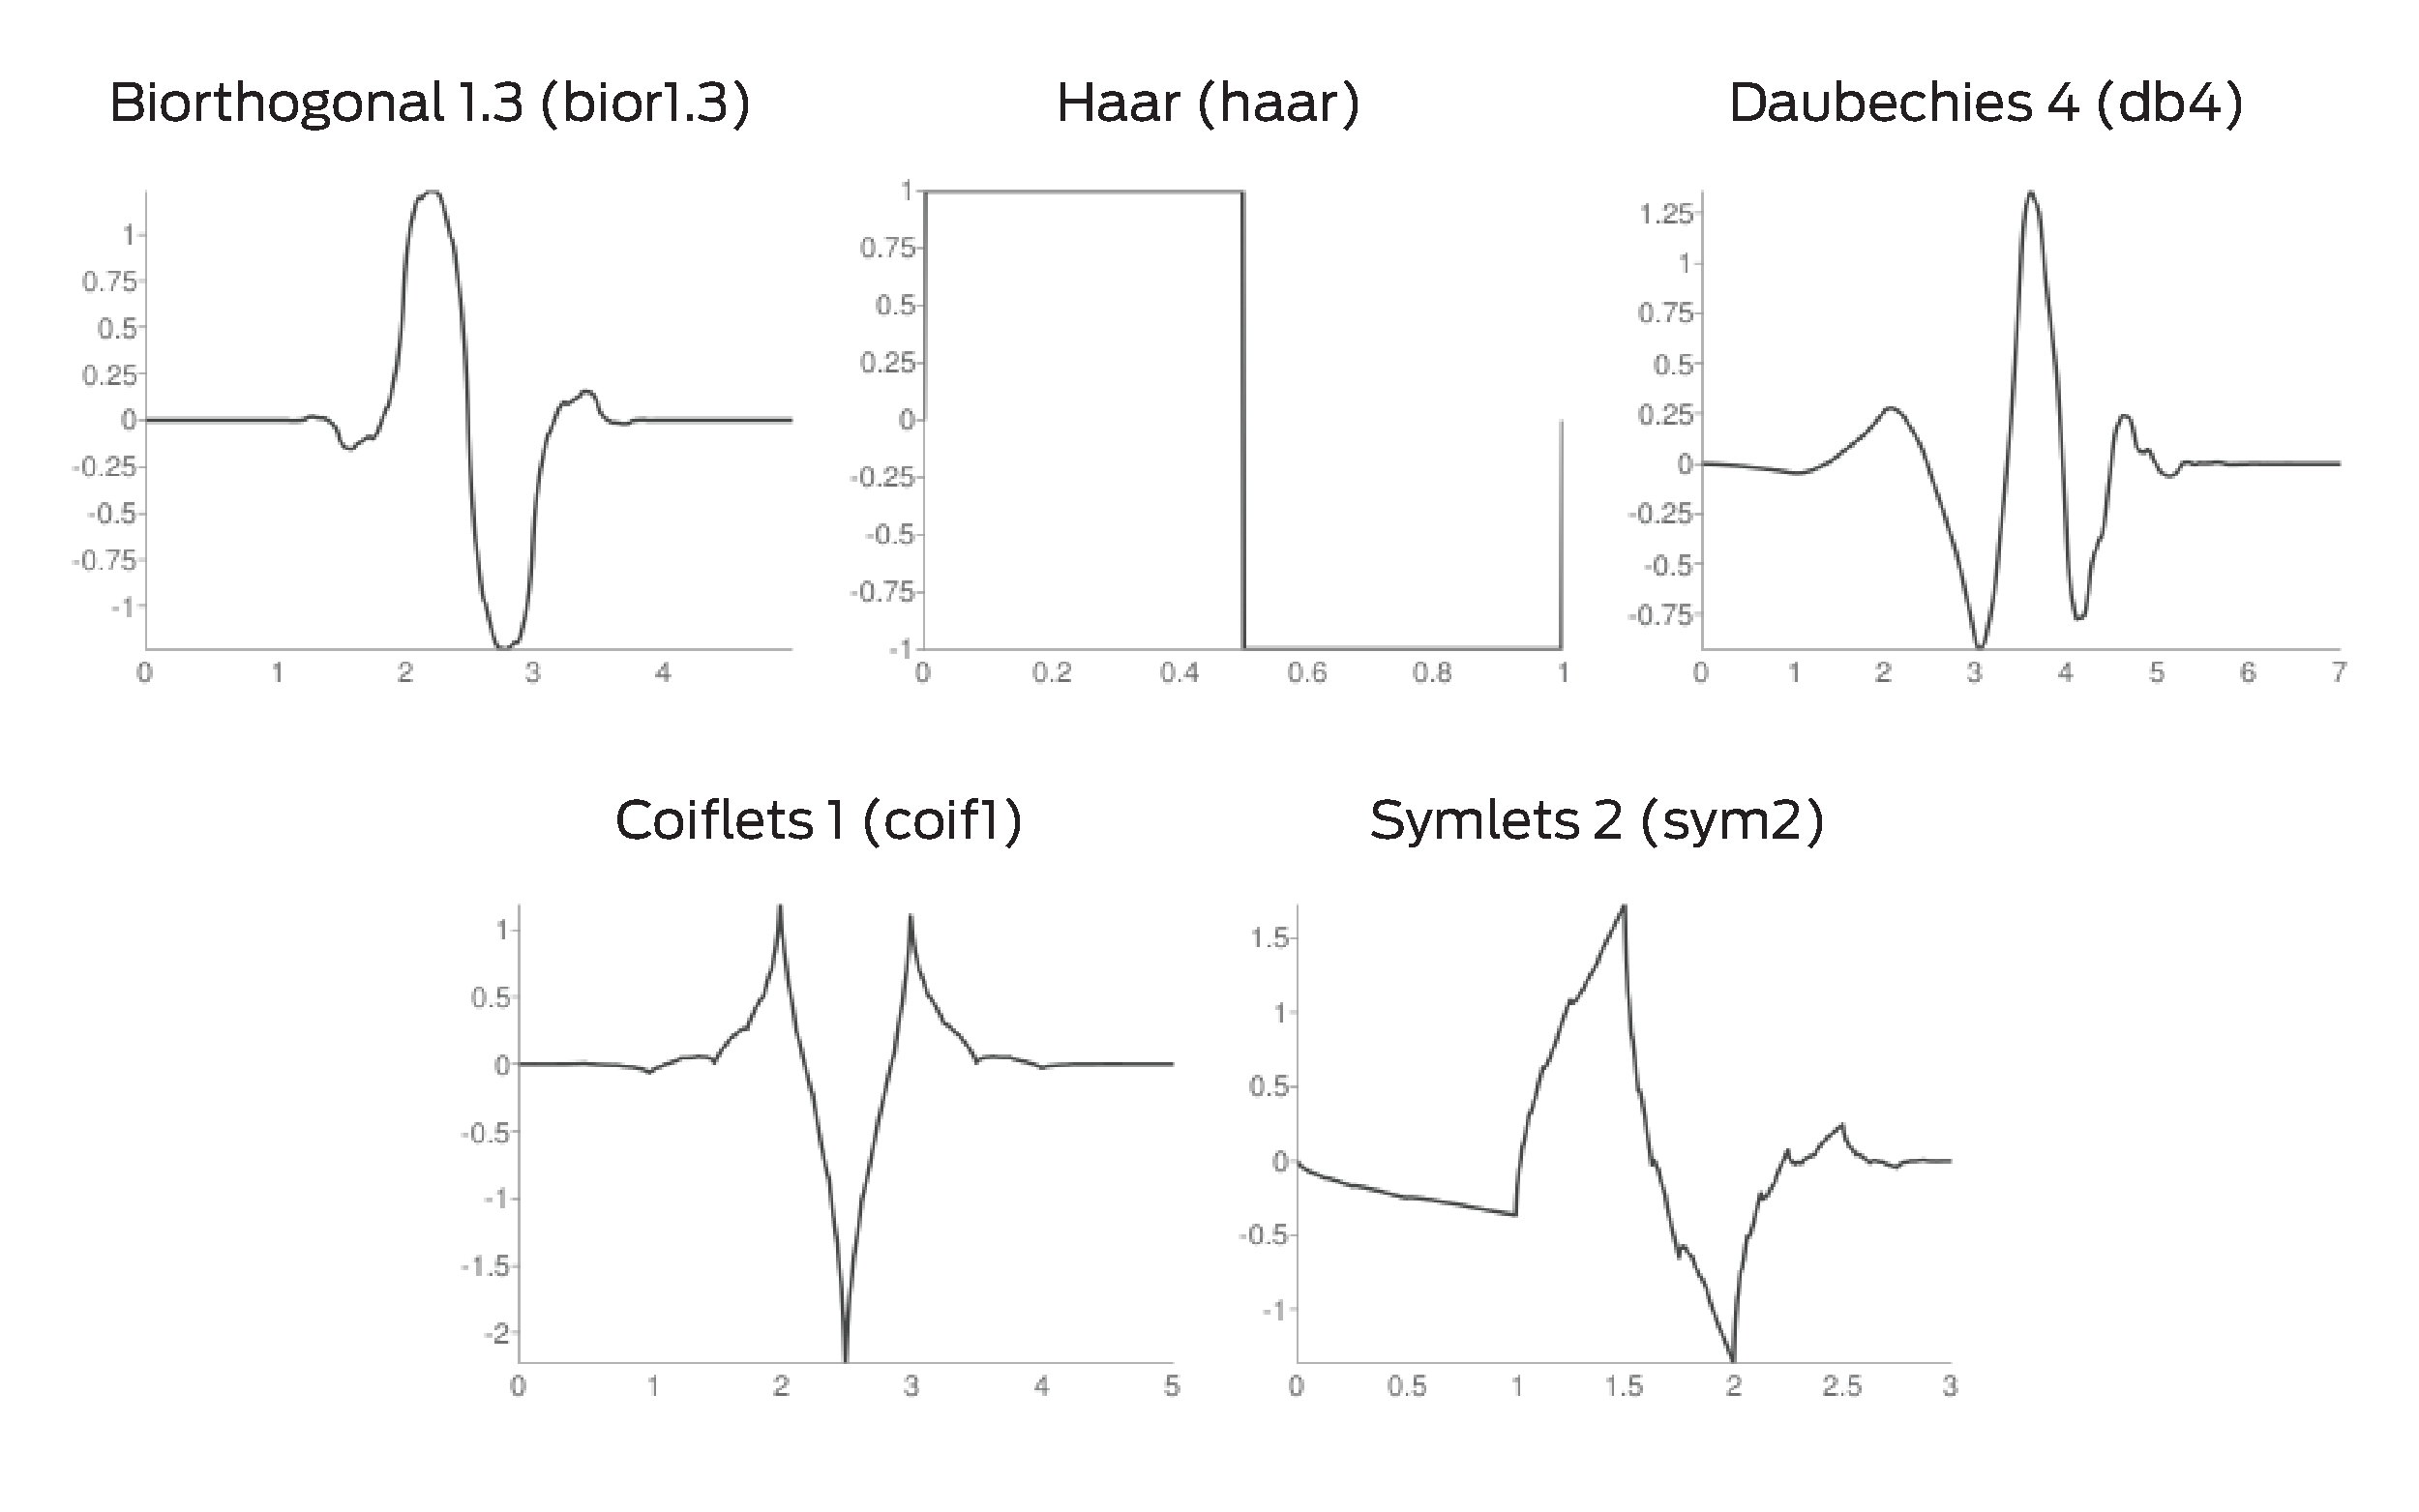
\includegraphics[width=0.8\textwidth]{images/report/wavelets.pdf}
\caption{Valčki uporabljeni pri testiranju}
\label{wavelets}
\end{center}
\end{figure}

Kot oceno najboljšega valčka za posamezno sliko sem vzel mero $P_{cc} >=0.99$ (Pearsonova korelacija) in $NRMSE <=0.07$. Razlog izbire teh mej je (subjektivna) ocena kakovosti slike in (večinoma) kompresijsko razmerje. V naslednjih podpoglavjih so izpostavljene tri najbolše kombinacije valčkov, pragovnih vrednosti in metode pragovne funkcije za posamezno sliko. Prednost imajo tiste kombinacije, ki nudijo višje kompresijsko razmerje. Primerjamo tudi kako se obnesejo te kombinacije v kolikor obrnemo metodo pragovne funkcije.

\subsection{Slika A}

\begin{figure}
\centering
\begin{subfigure}[t]{0.8\textwidth}

\includegraphics[width=1\textwidth]{images/adventuretime.jpg}
\caption{Slika iz risanke, veliko ostrih prehodov barv.}
\label{slika1}
\end{subfigure}
\centering
\begin{subfigure}[t]{0.8\textwidth}

\includegraphics[width=1\textwidth]{images/report/adventuretime_comp.jpg}
\caption{Slika risanke, stisnjena s Haarovim valčkom, pragovno vrednostjo 20, 9 nivojev dekompozicije in mehka pragovna funkcija.}
\label{slika1:comp}
\end{subfigure}
\end{figure}


\begin{verbatim}
TOP 3 metrics from metrics/adventuretime_metrics.csv
 Wavelet  Threshold	Levels	Mode		 Pearson cor.	   	   NRMSE	    Compression
   haar	         20	     9	soft	     0.996404     0.044135	   	  1.785614
   haar	         20	     4	soft	     0.996408     0.044738	   	  1.785490
   haar	         50	     4	hard	     0.995147     0.049986	   	  1.634995

Conditions: Pearson >= 0.99	and	NRMSE <= 0.07
\end{verbatim}

Pri sliki~\ref{slika1} se je izkazalo, da jo s pomočjo Haarovega valčka še lahko stisnemo brez prevelikih izgub (slika~\ref{slika1:comp}). V kolikor zamenjamo pragovno metodo:
\begin{verbatim}
Wavelet  Threshold	Levels	Mode		 Pearson cor.	   NRMSE  Compression
  haar	         20	     9	hard	      0.9989    0.0241	   	  1.5740
\end{verbatim}
Vidimo, da se napaka (NRMSE) skoraj prepolovi, v zameno pa izgubimo $11.8\%$ kompresije.

\subsection{Slika B}

\begin{figure}
\centering
\begin{subfigure}[t]{0.8\textwidth}
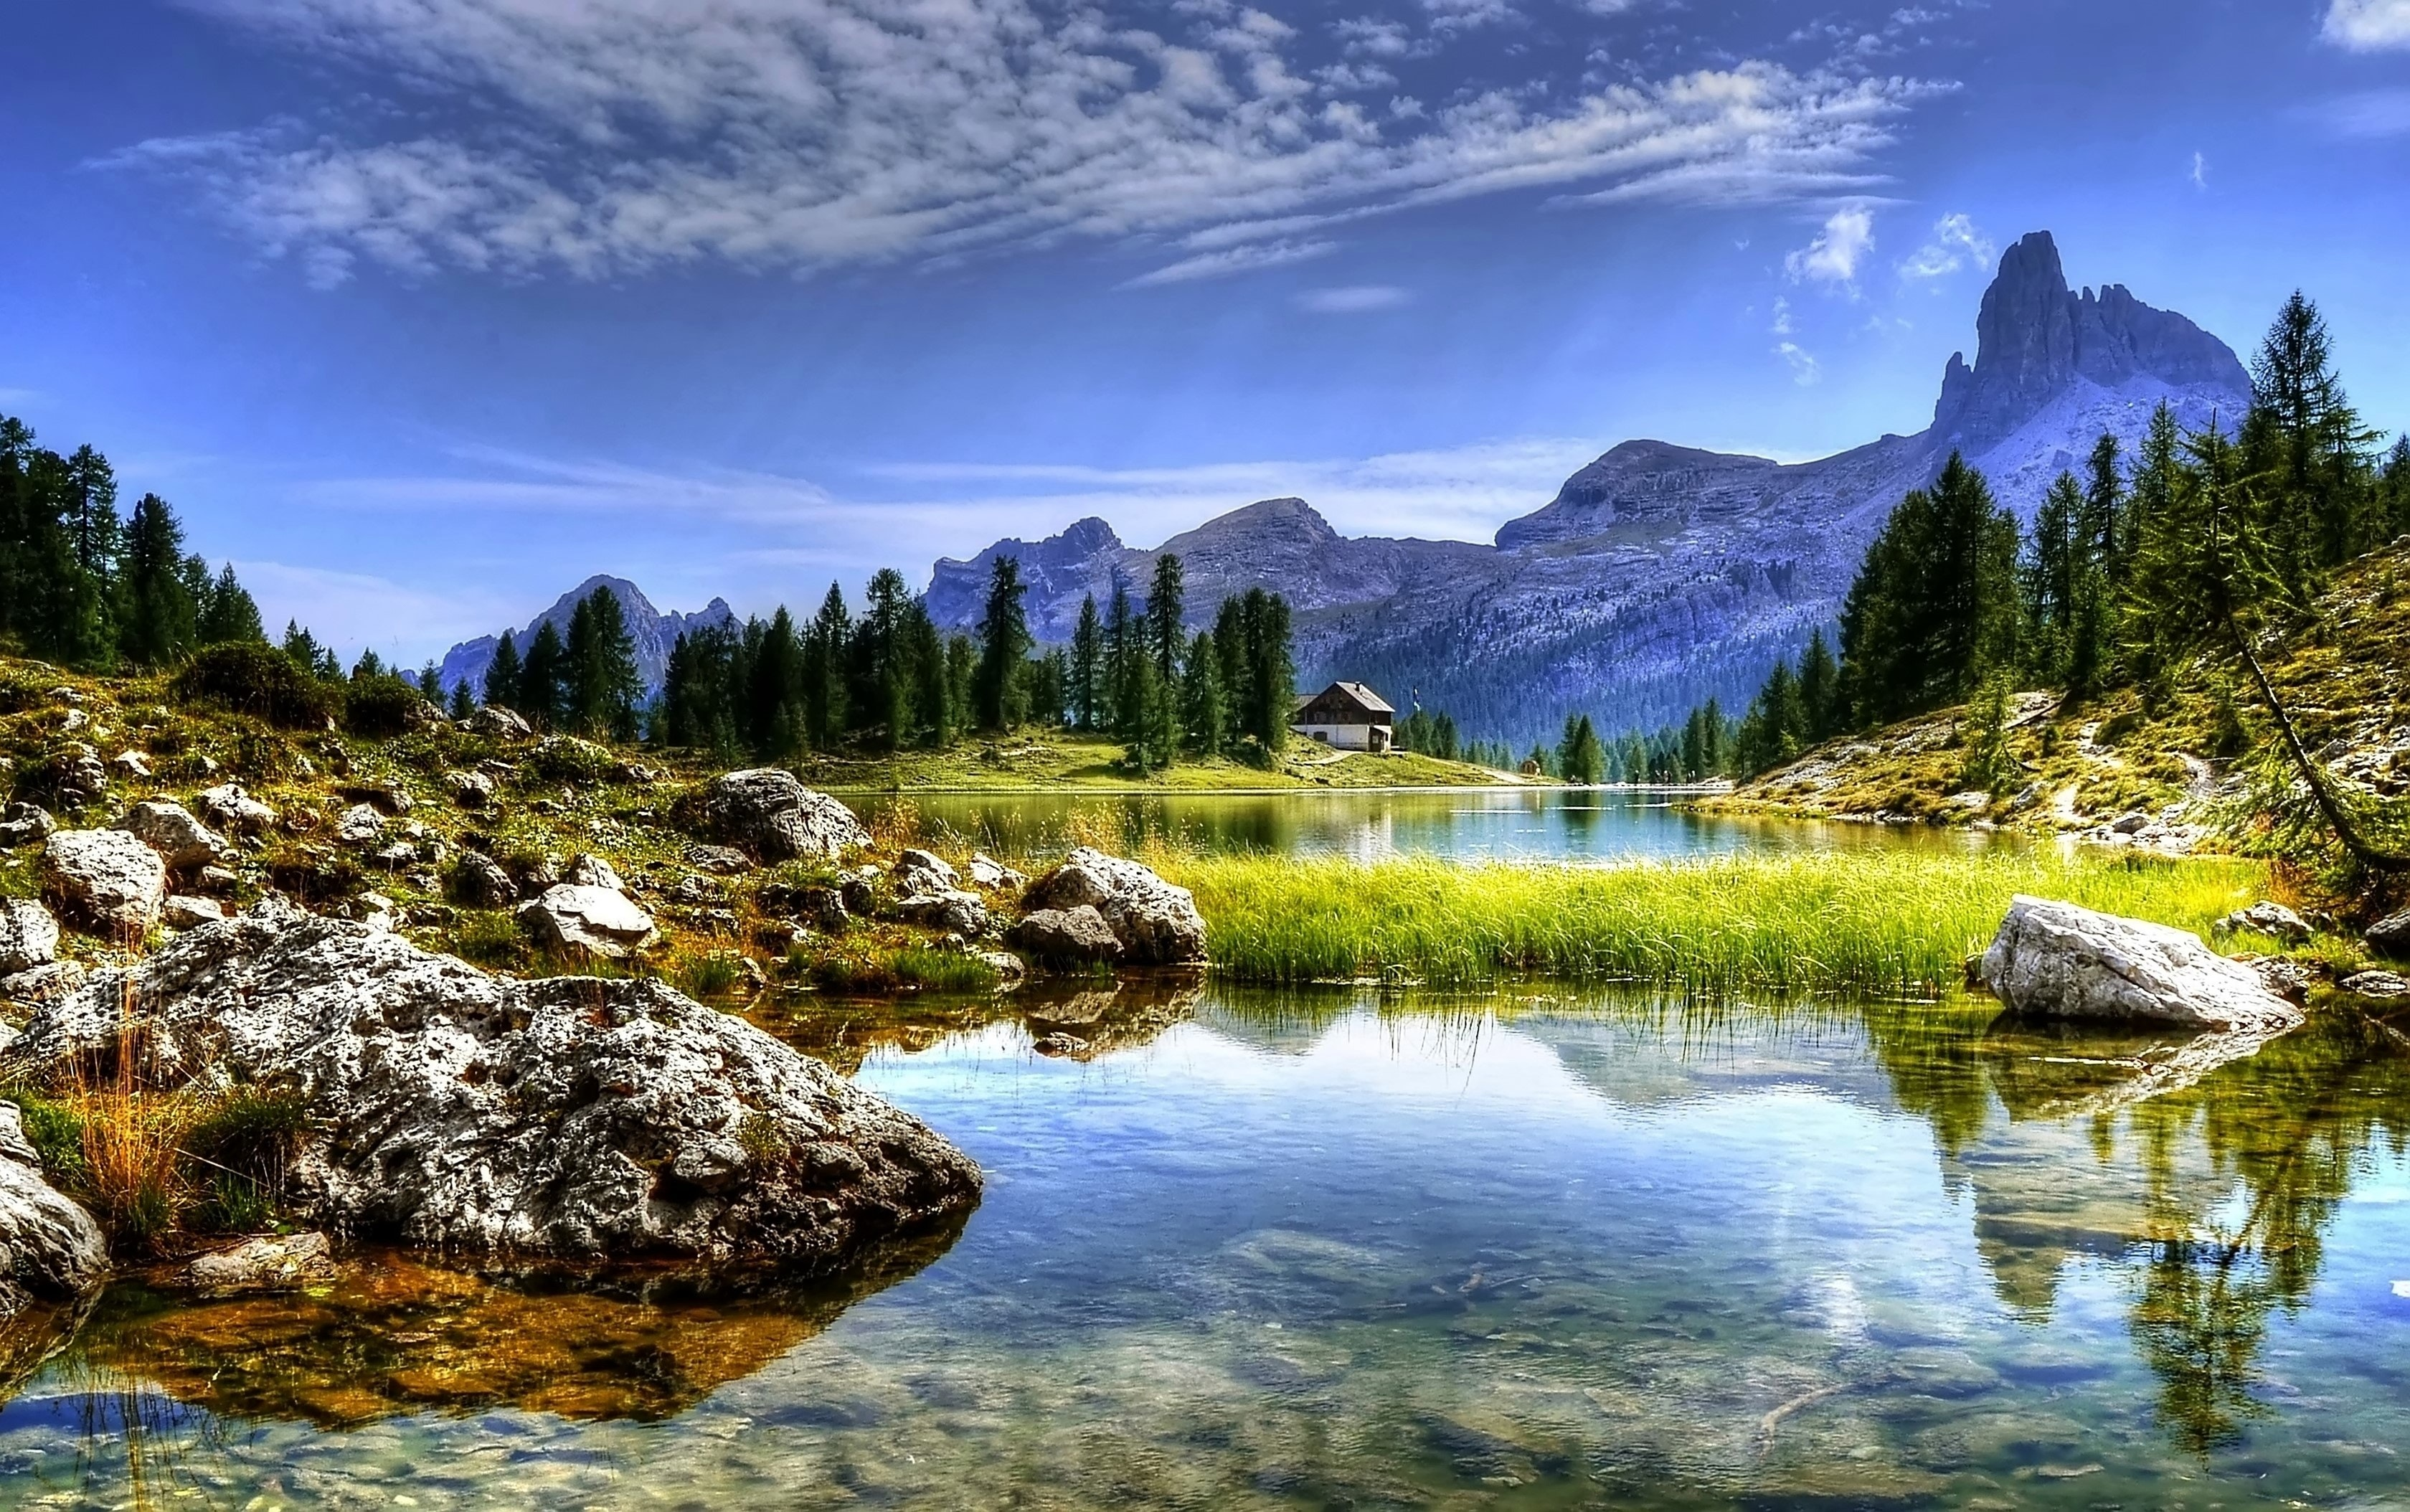
\includegraphics[width=1\textwidth]{images/country.jpg}
\caption{Slika pokrajine.} \label{slika2}
\end{subfigure}
\centering
\begin{subfigure}[t]{0.8\textwidth}
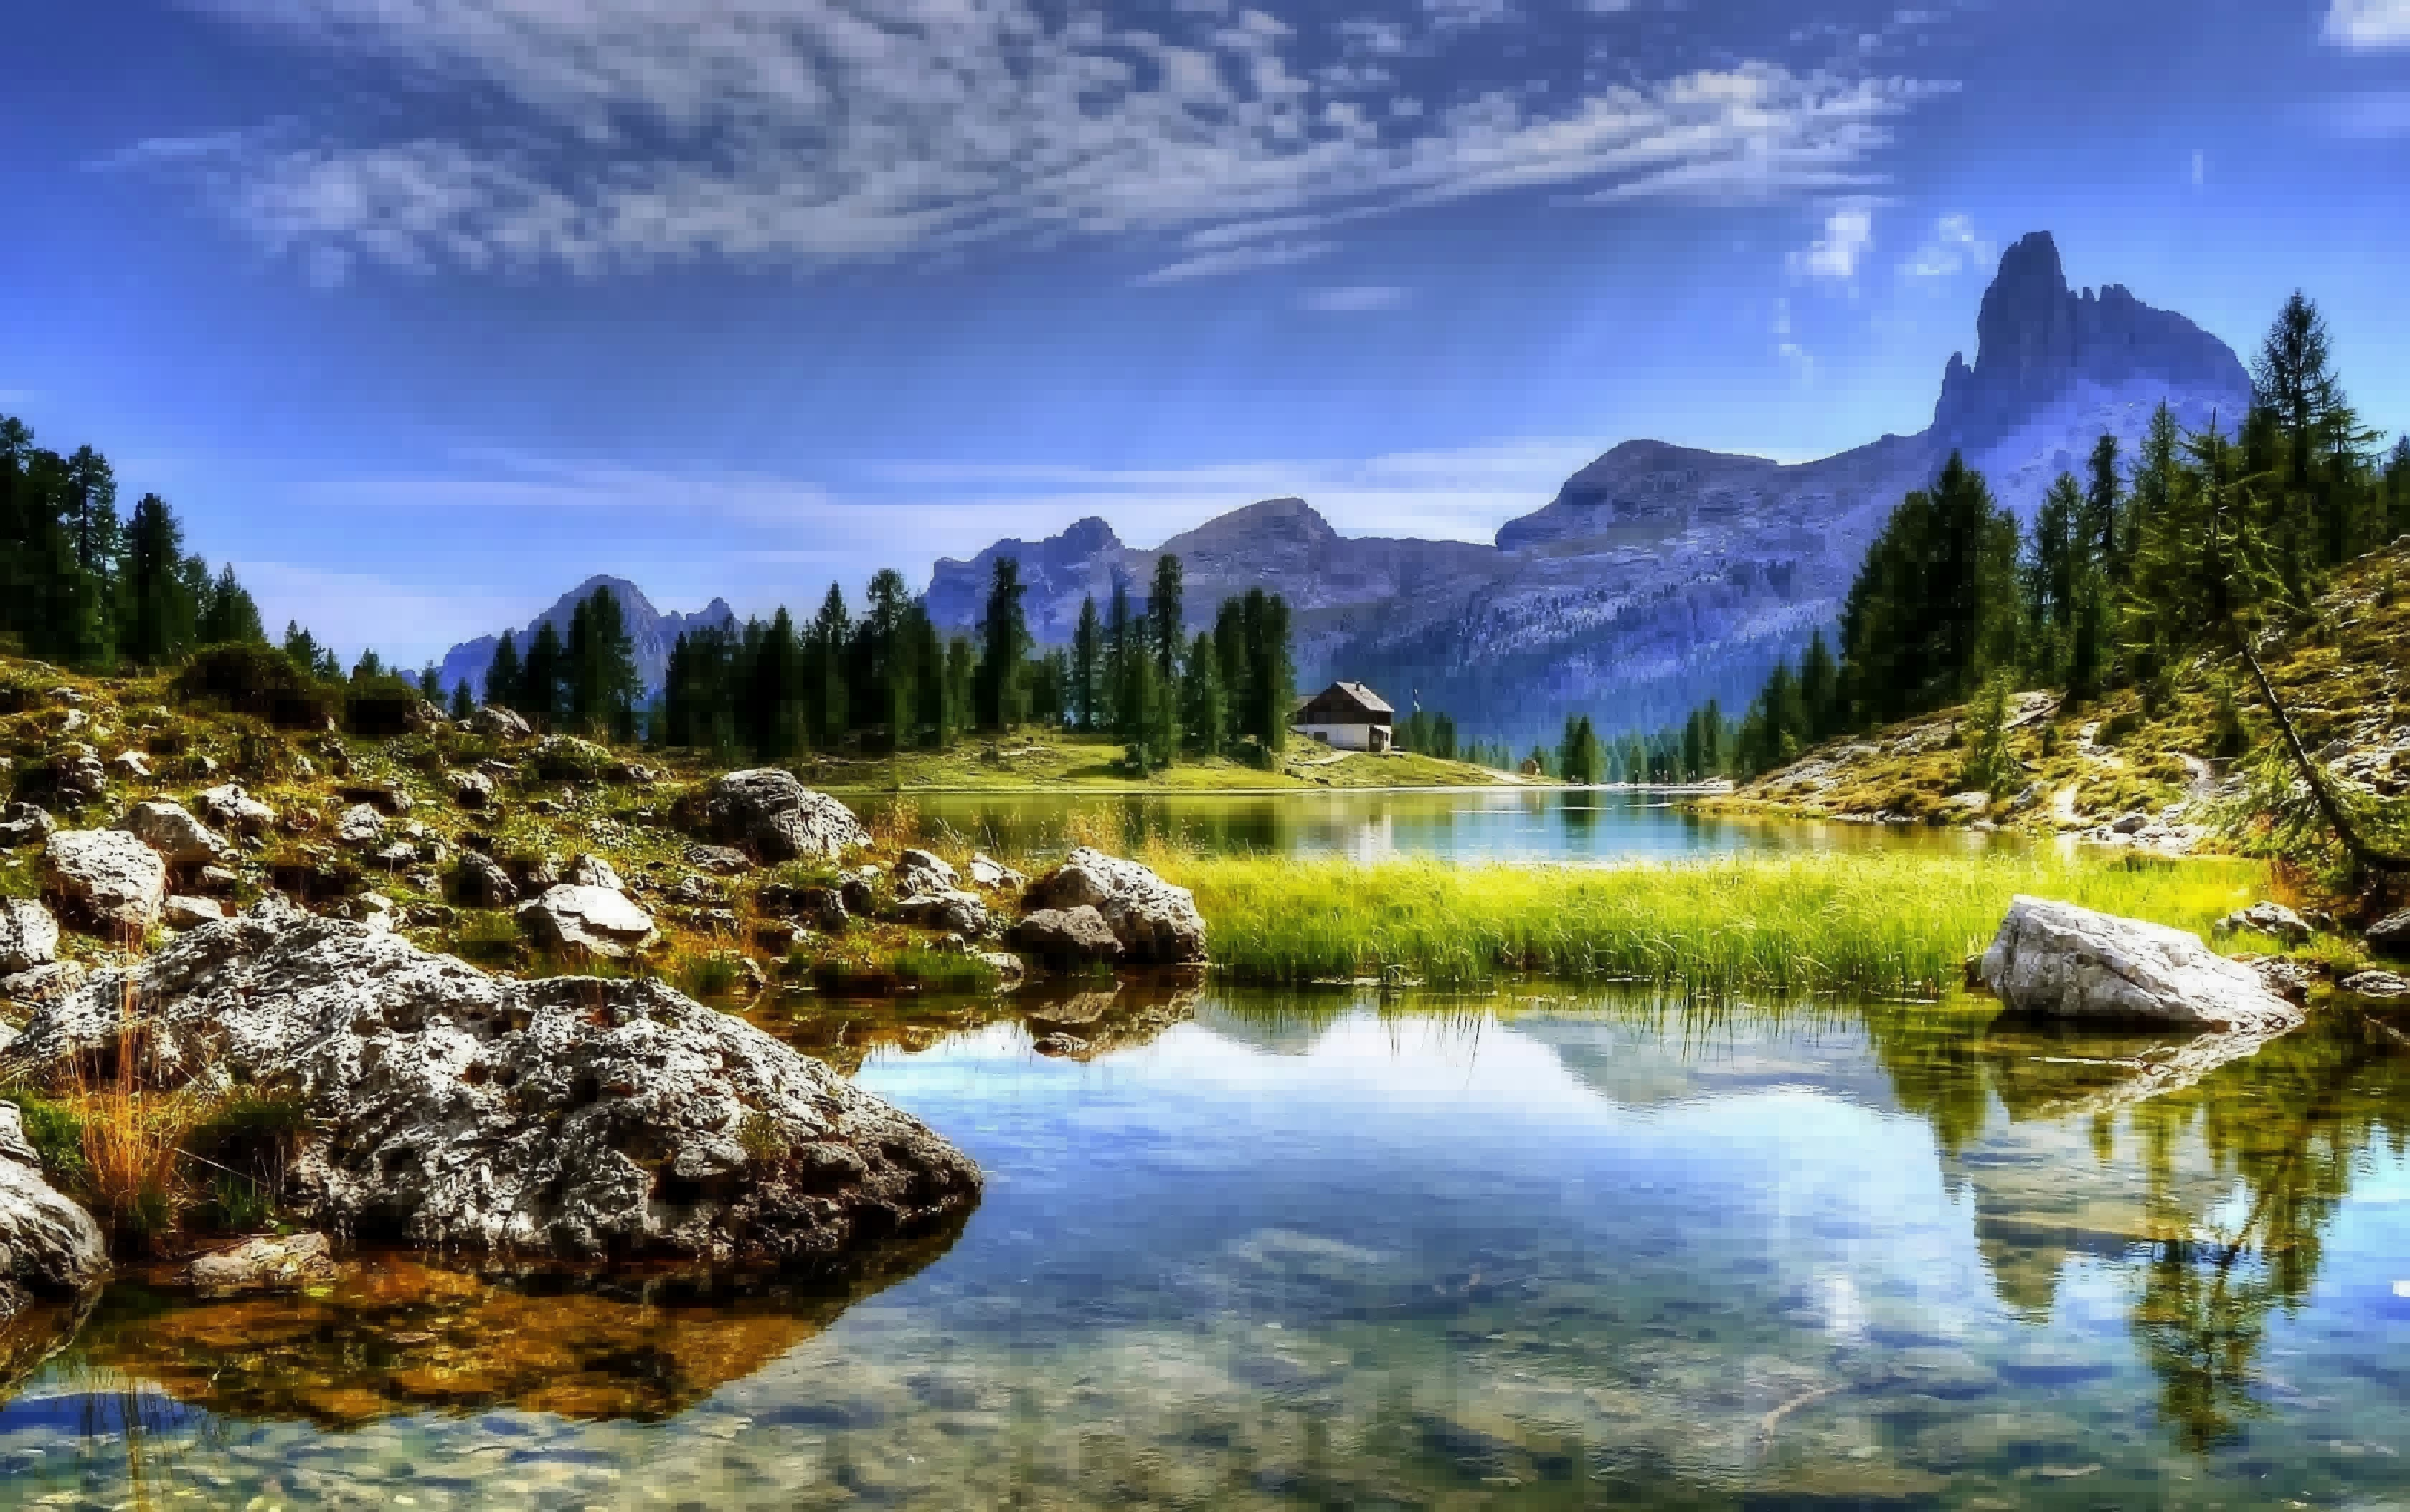
\includegraphics[width=1\textwidth]{images/report/country_comp.jpg}
\caption{Slika pokrajine, stisnjena s Haarovim valčkom, pragovno vrednostjo 50, 4 nivoji dekompozicije in mehka pragovna funkcija.}
\label{slika2:comp}
\end{subfigure}
\end{figure}

\begin{verbatim}
TOP 3 metrics from metrics/country_metrics.csv
	Wavelet	Threshold	Levels	Mode	Pearson cor.	   NRMSE 	Compression
	    db4	       20	     9	soft	    0.993602 	0.068033	   0.766180
	    db4	       20	     4	soft	    0.993646 	0.068820	   0.764033
	   haar	        2	     4	soft	    0.999769 	0.012966	   0.703736

Conditions: Pearson >= 0.99	and	NRMSE <= 0.07
\end{verbatim}

Slika~\ref{slika2} je bila zanimiva, saj z enakimi koeficienti, ki so drugje stisnili slike, brez prevelikih napak, tukaj povzročijo večjo sliko. Prva stisnjena slika je pri $P_{cc} >= 0.97$ in $NRMSE <= 0.15$, Haarov valček. 
\begin{verbatim}
TOP 3 metrics from metrics/country_metrics.csv
	Wavelet	Threshold	Levels	Mode	Pearson cor.	    NRMSE	Compression
	   haar	       50	     9	soft	    0.975114 	0.133222	   1.109410
	   haar	       50	     4	soft	    0.975455 	0.137268	   1.108318
	    db4	       50	     9	soft	    0.980862 	0.117146	   0.890775

Conditions: Pearson >= 0.9	and	NRMSE <= 0.15
\end{verbatim}
Kar pa se tiče kakovosti, pa lahko presodite sami na sliki~\ref{slika2:comp}. V kolikor obrnemo pragovno funkcijo na trdo, dobimo naslednje rezultate:
\begin{verbatim}
 Pearson correlation:	0.9879
 Normalized RMSE:		0.0915
 Compression ratio:		0.7809
\end{verbatim}
V tem primeru izgubimo kompresijo in smo poleg poslabšanja kakovosti vnesli tudi večjo velikost slike.


\subsection{Slika C}

\begin{figure}
\begin{subfigure}[t]{0.48\textwidth}
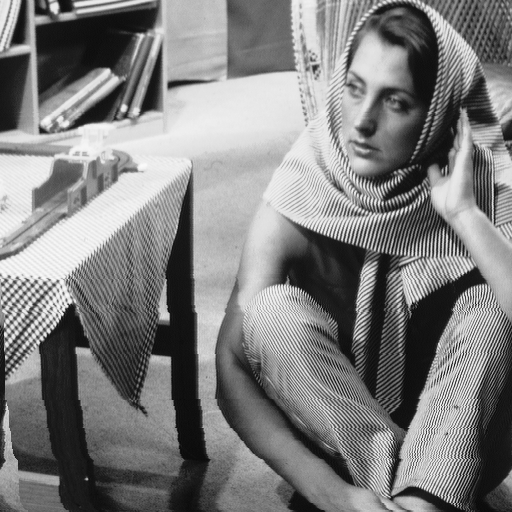
\includegraphics[width=1\textwidth]{images/barbara_gray.png}
\caption{Sivinska slika.} \label{slika3}
\end{subfigure}
\hspace*{\fill} % separation between the subfigures
\begin{subfigure}[t]{0.48\textwidth}
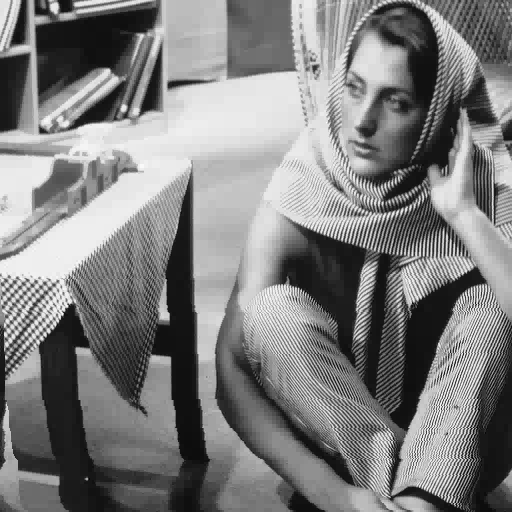
\includegraphics[width=1\textwidth]{images/report/barbara_gray_comp.png}
\caption{Sivinska slika stisnjena s Haarovim valčkom, pragovno vredost 20, 9 nivojev dekompozicije in trdo pragovno funkcijo.} \label{slika3:comp}
\end{subfigure}
\end{figure}

\begin{verbatim}
TOP 3 metrics from metrics/barbara_gray_metrics.csv
	Wavelet	Threshold	Levels	Mode	Pearson cor.	    NRMSE	Compression
	   haar	       20	     9	hard	    0.996536 	0.047337	   1.291171
	   haar	       20	     4	hard	    0.996539 	0.047320	   1.290339
	bior1.3	       20	     9	hard	    0.996514 	0.047516	   1.197921

Conditions: Pearson >= 0.99	and	NRMSE <= 0.07
\end{verbatim}
Tudi sivinska slika~\ref{slika3} se je stisnila (slika~\ref{slika3:comp}) pod podanimi pogoji. V kolikor obrnemo pragovno funkcijo:
\begin{verbatim}
 Pearson correlation:	0.9889
 Normalized RMSE:		0.0877
 Compression ratio:		1.3639
\end{verbatim}
dobimo $5.7\%$ boljše kompresijsko razmerje, poveča pa se napaka za $86\%$.

\subsection{Slika D}

\begin{figure}
\begin{subfigure}[t]{0.48\textwidth}
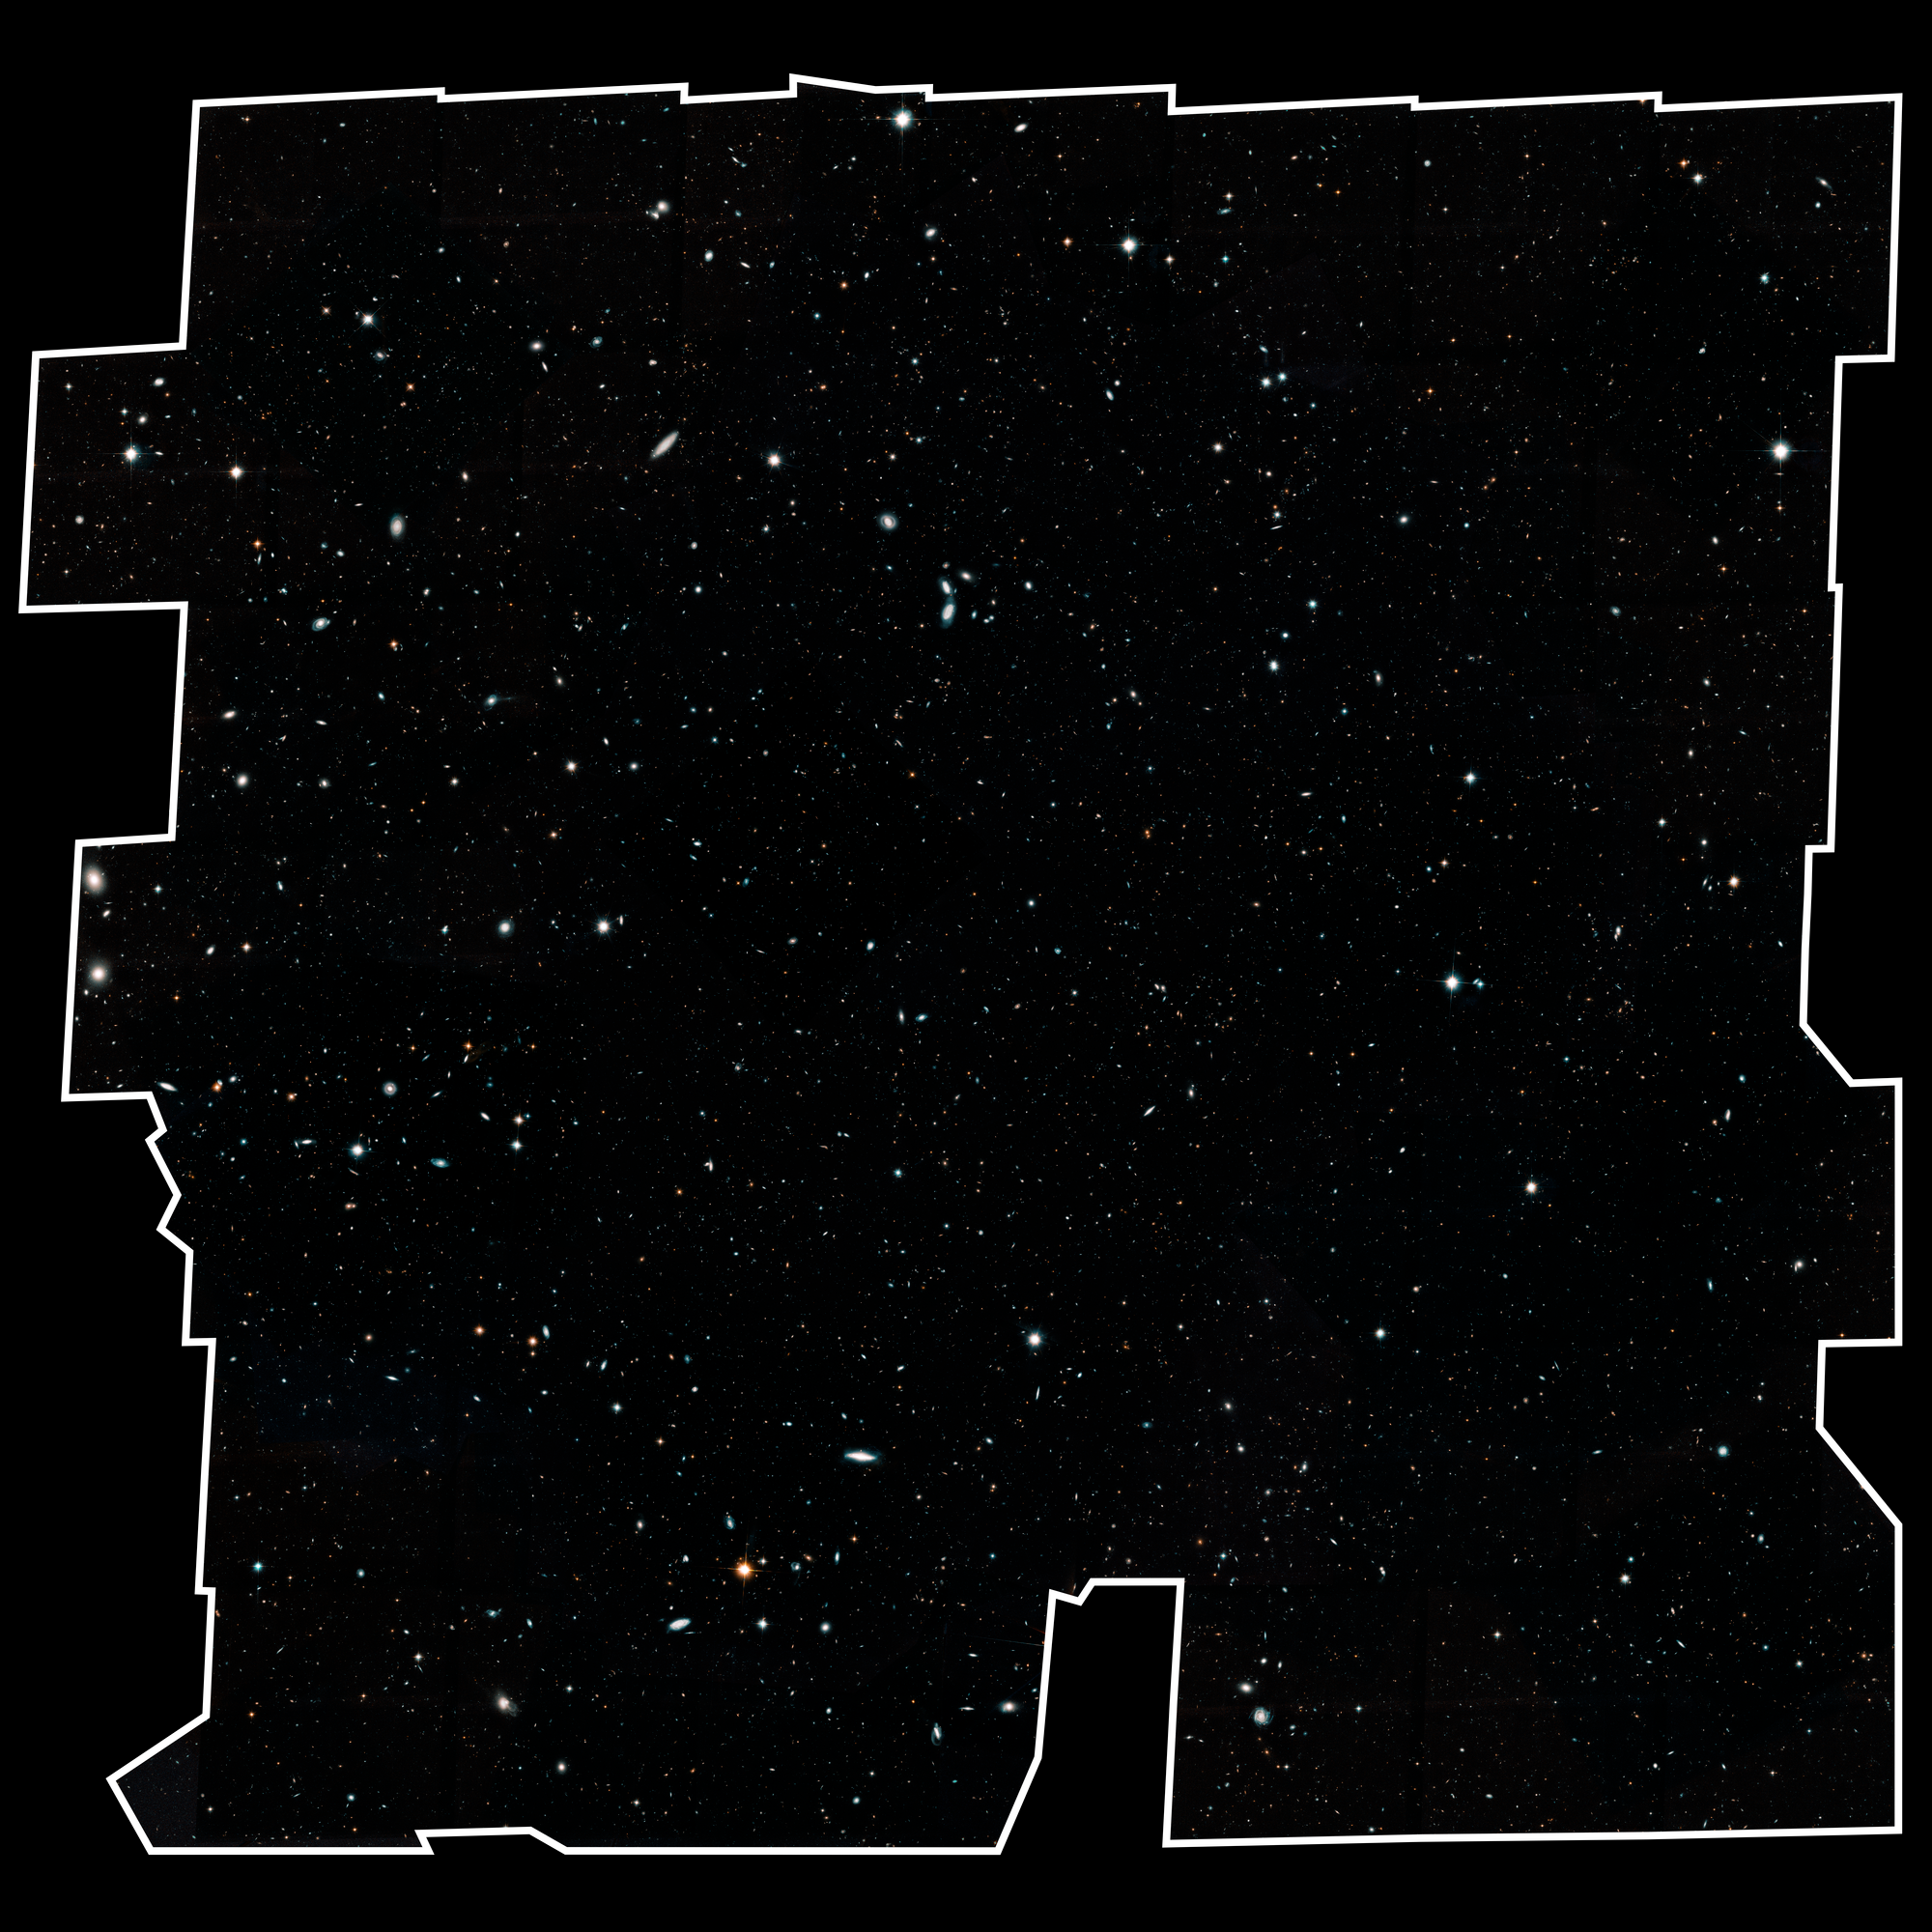
\includegraphics[width=1\textwidth]{images/hubble2000x2000.png}
\caption{Slika vesolja (Hubble), pomembno je ohraniti majhne zvezde.} \label{slika4}
\end{subfigure}
\hspace*{\fill} % separation between the subfigures
\begin{subfigure}[t]{0.48\textwidth}
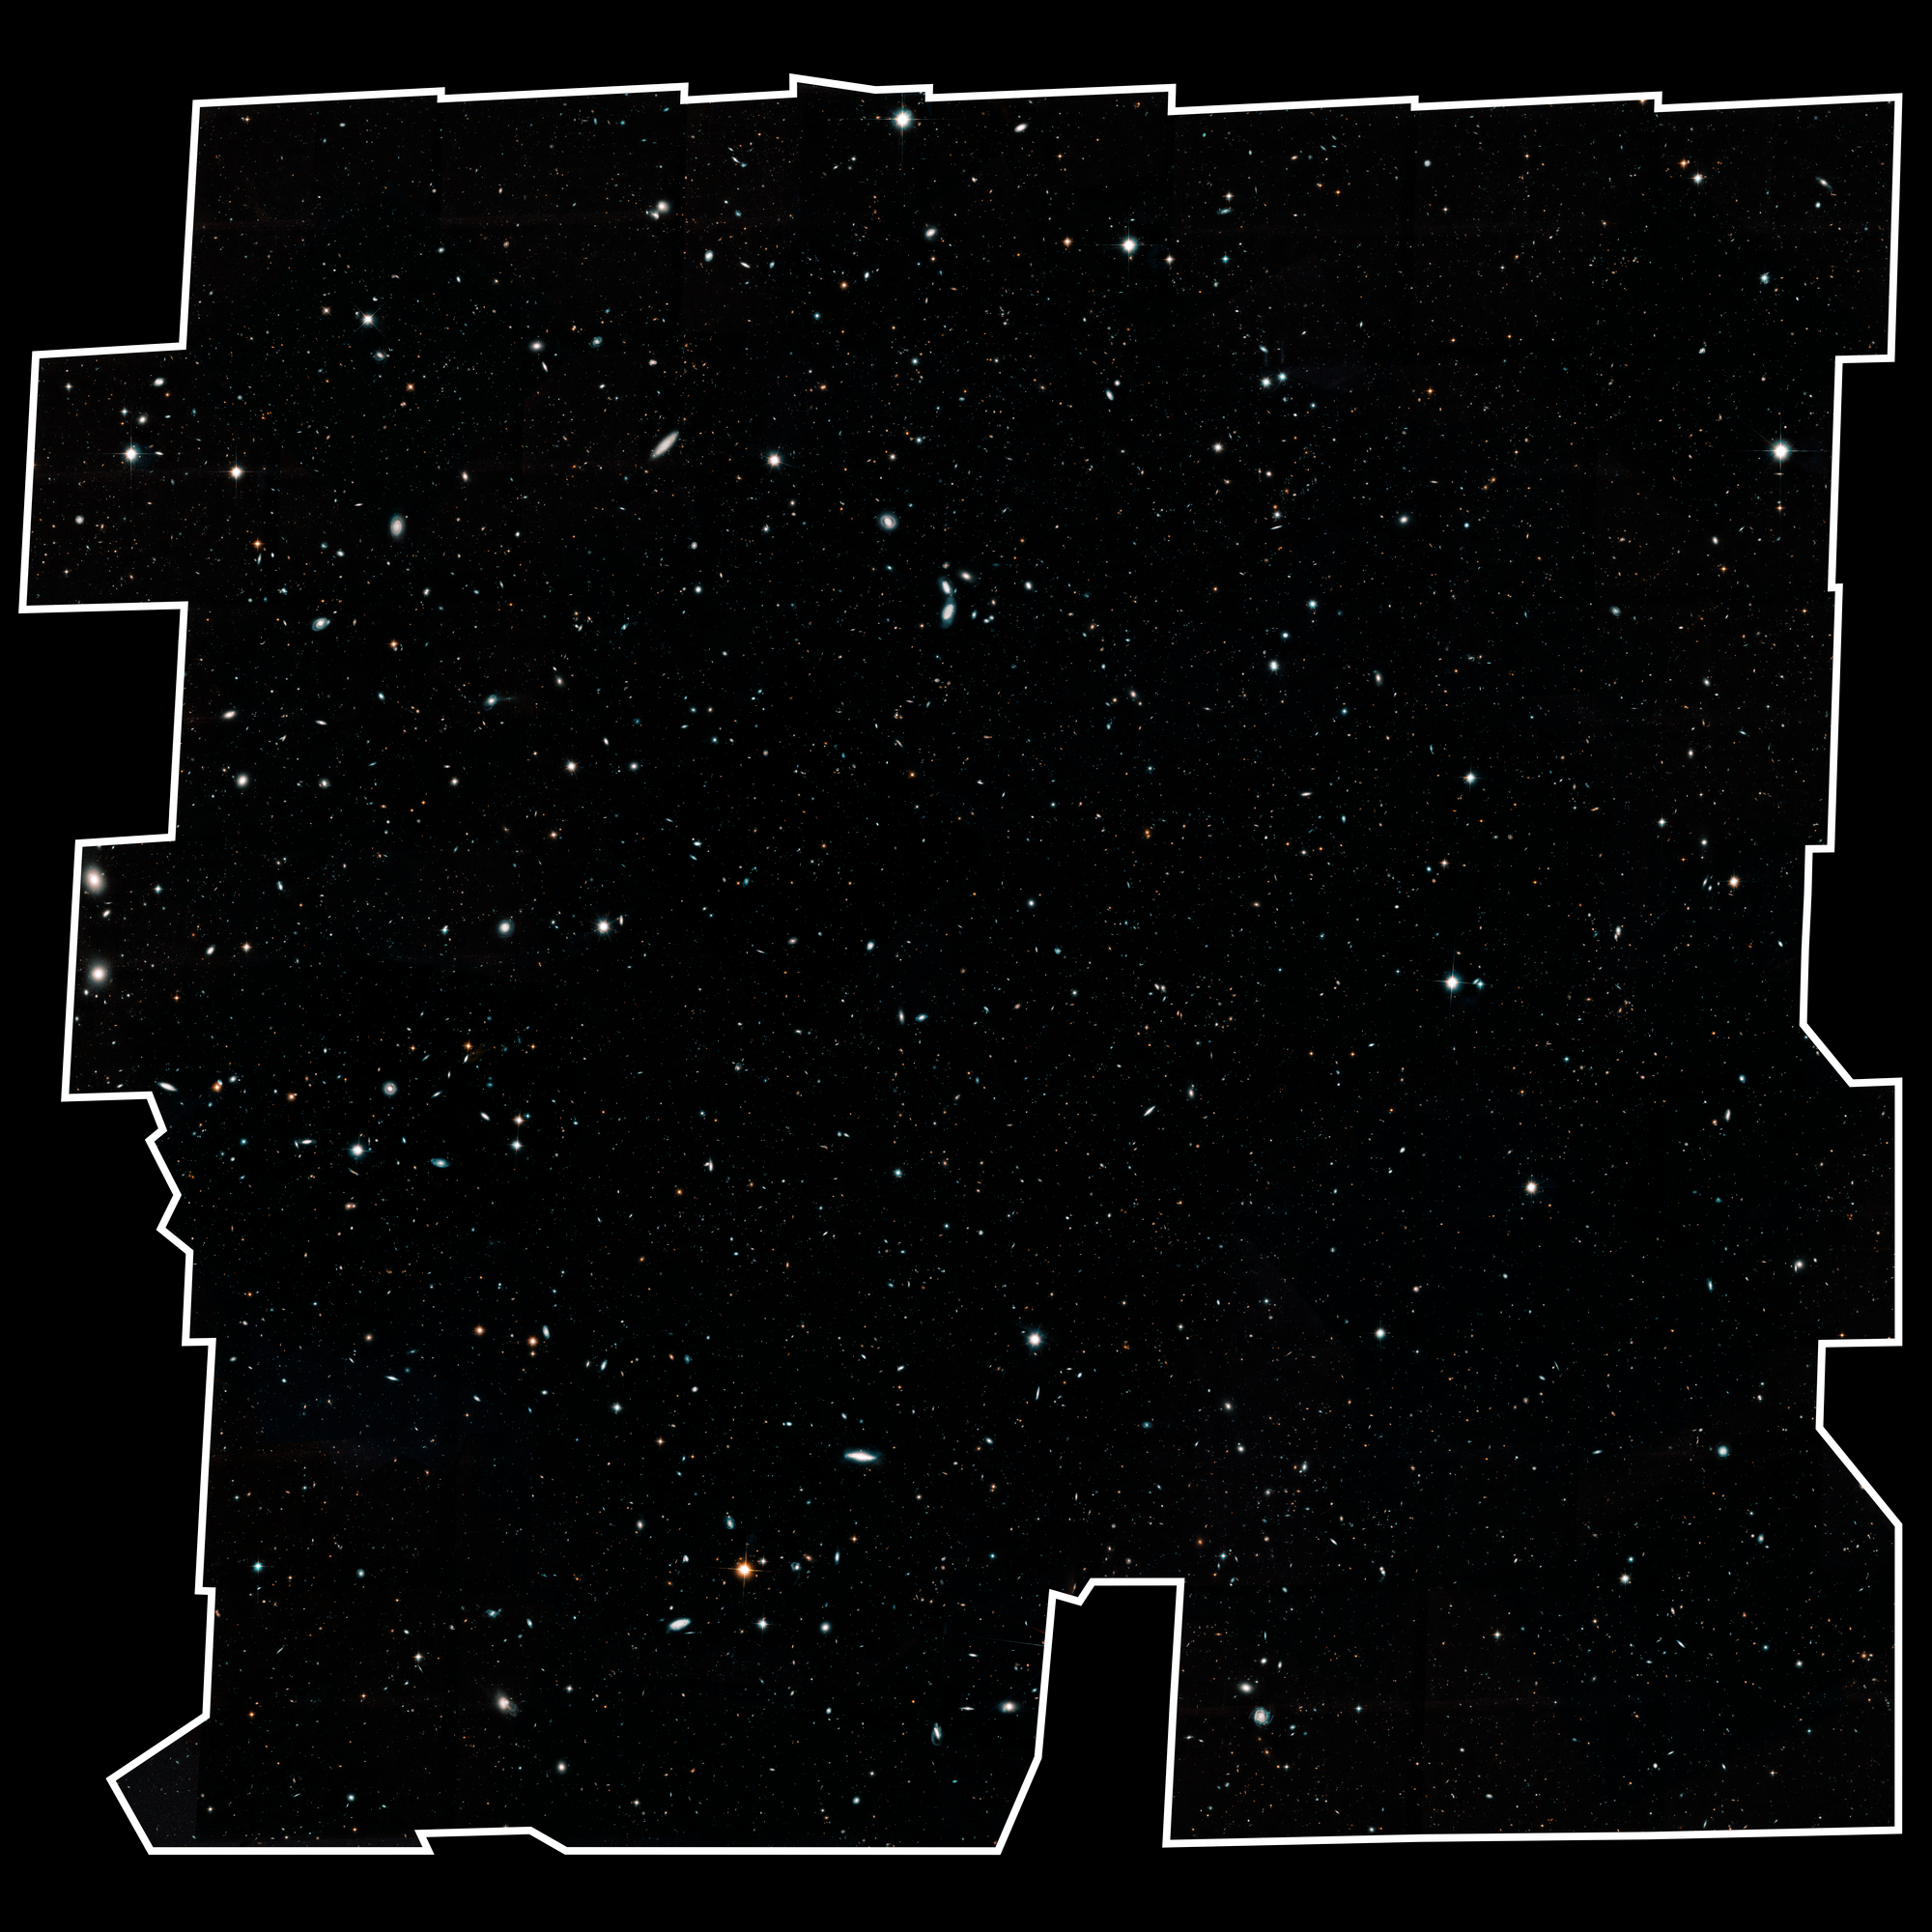
\includegraphics[width=1\textwidth]{images/report/hubble2000x2000_comp.png}
\caption{Slika vesolja stisnjena s Haarovim valčkom, pragovno vredost 2, 9 nivojev dekompozicije in trdo pragovno funkcijo.} \label{slika4:comp}
\end{subfigure}
\end{figure}

\begin{verbatim}
TOP 3 metrics from metrics/hubble2000x2000_metrics.csv
	Wavelet	Threshold	Levels	Mode 	Pearson cor.	   NRMSE 	Compression
	   haar	        2	     9	hard	    0.999881 	0.068949	   1.215071
	   haar	        2	     4	hard	    0.999881 	0.068924	   1.214732
	   haar	        2	     1	hard	    0.999901 	0.063717	   1.076047

Conditions: Pearson >= 0.99	and	NRMSE <= 0.07
\end{verbatim}
Pri sliki vesolja smo zopet na meji stiskanja, najboljše rezultate pa daje Haarov valček s pragovno vrednostjo 2. Če obrnemo pragovno funkcijo na mehko, dobimo naslednje rezultate:
\begin{verbatim}
 Pearson correlation:	0.9996
 Normalized RMSE: 		0.1341
 Compression ratio: 		1.4491
\end{verbatim}
Kompresijsko razmerje je boljše za $19\%$, medtem ko se napaka NRMSE skoraj podvoji.

\subsection{Šumna slika}

Sliki~\ref{slika1} sem dodal $SNR=20dB$ šuma (\textit{white\_noise.py}) in sem dobil novo sliko~\ref{noisy}. Primerjane vrednosti za $P_{cc}$ in $NRMSE$ se štejejo glede na prvotno sliko~\ref{slika1}. Razmerje stiskanja pa ostaja med šumno sliko in dodatno obdelano šumno sliko, saj se je ob dodajanju šuma povečala velikost izvorne slike.
Metrike sortirane glede na najmanjši NRMSE:
\begin{verbatim}
TOP 3 metrics from metrics/noisy_metrics.csv
	Wavelet	Threshold	Levels	Mode	Pearson cor.	   NRMSE 	Compression
	  coif1	      150	     4	hard	    0.942010 	0.207928	   2.073749
	    db4	      150	     4	hard	    0.941066 	0.208361	   2.054643
	  coif1	      150	     9	hard	    0.941701 	0.208553	   2.084514
\end{verbatim}
Metrike sortirane glede na največji Pearsonov korelacijski koeficient:
\begin{verbatim}
TOP 3 metrics from metrics/noisy_metrics.csv
	Wavelet	Threshold	Levels	Mode	Pearson cor.	   NRMSE 	Compression
	    db4	      150	     4	soft	    0.960003 	0.245710	   4.205527
	  coif1	      150	     4	soft	    0.958285 	0.248087	   3.994817
	   sym2	      150	     4	soft	    0.958226 	0.248158	   3.958366
\end{verbatim}
Primerjava vseh štirih slik je na voljo na sliki~\ref{noisy:cmp}.


\begin{figure}
\begin{subfigure}[t]{0.48\textwidth}

\includegraphics[width=1\textwidth]{images/adventuretime.jpg}
\caption{Risana slika, izvirnik.} \label{noisy:origin}
\end{subfigure}
\hspace*{\fill} % separation between the subfigures
\begin{subfigure}[t]{0.48\textwidth}

\includegraphics[width=1\textwidth]{images/noisy.jpg}
\caption{Risana slika z dodanim $20dB$ šumom.} \label{noisy}
\end{subfigure}

\begin{subfigure}[t]{0.48\textwidth}

\includegraphics[width=1\textwidth]{images/report/noisy_nrmse_comp.jpg}
\caption{Šumna slika obdelana s Coiflet 1 valčkom, pragovno vredost 150, 4 nivoji dekompozicije in trdo pragovno funkcijo.} \label{noisy:comp:nrmse}
\end{subfigure}
\hspace*{\fill} % separation between the subfigures
\begin{subfigure}[t]{0.48\textwidth}

\includegraphics[width=1\textwidth]{images/report/noisy_pearson_comp.jpg}
\caption{Šumna slika obdelana s Daubechies 4 valčkom, pragovno vredost 150, 4 nivoji dekompozicije in mehko pragovno funkcijo.} \label{noisy:comp:pearson}
\end{subfigure}
\label{noisy:cmp}
\end{figure}

\end{document}
